\documentclass[a4paper,12pt]{report}
\usepackage[utf8]{inputenc}
\usepackage[T1]{fontenc}
\usepackage[english]{babel}
\usepackage{lmodern}

%hyperref for interactive PDF index
\usepackage[bookmarks, colorlinks, breaklinks]{hyperref}
\hypersetup{linkcolor=black, citecolor=black, filecolor=black, urlcolor=black}

%Package required to use special symbols
\usepackage{amsmath, amssymb}

%tPackage for tables
\usepackage{tabu}
\usepackage{tabularx}
\usepackage{ltablex}
\usepackage{longtable}
\usepackage{float} % To allow the use of H modifier in long tables

%Package required to use figures
\usepackage{graphicx}
%Include the bibliography in the table of contents
\usepackage{tocbibind}

%Package used to insert figures at the specified position
\usepackage{float}

%Packages for Alloy code listing
\usepackage{listings}
\usepackage{alloy}
\usepackage{color}
\definecolor{alloy-keyword}{rgb}{0.23, 0.23, 0.7}
\definecolor{alloy-comment}{rgb}{0.18, 0.64, 0.18}
\definecolor{alloy-string}{rgb}{0.71, 0.18, 0.71}

%To call Chapters -> Sections
\addto\captionsenglish{\renewcommand{\chaptername}{Section}}

%To have a new line after a \paragraph
\newcommand{\myparagraph}[1]{\paragraph{#1}\mbox{}\\}

%References Packages
\usepackage{xr-hyper}
\usepackage{hyperref}

\begin{document}

%Title page
\begin{titlepage}
\centering
	\begin{center}{
		\begin{figure}[h]
		\large
		\centering
		{
\includegraphics[width=.60\linewidth]{img/logo_poli}}
        \end{figure}
    	}
	\end{center}
	\vspace{1 cm}
	{\Large {\textbf{\LARGE TrackMe} \\
		Software Engineering II - Prof. Elisabetta Di Nitto} \par}
	\vspace{1.5cm}
	{\LARGE \textbf{Requirements Analysis and Specification Document} \par}
	\vspace{1.5cm}
	{\Large\itshape Michele Gatti, Federica Gianotti, Mathyas Giudici\par}
	\vspace{2cm}
	\vfill
	% Bottom of the page
	{\large Document version: 1.0\par}
	{\large \today \par}
\end{titlepage}

{
\begin{table}[h!]
\begin{tabu} to \textwidth { X[0.3,r,p] X[0.7,l,p] }
\textbf{Deliverable:} & RASD\\
\textbf{Title:} & Requirement Analysis and Specification Document \\
\textbf{Authors:} & Michele Gatti, Federica Gianotti, Mathyas Giudici \\
\textbf{Version:} & 1.0 \\
\textbf{Date:} & \today \\
\textbf{Download page:} & https://github.com/MathyasGiudici/GattiGianottiGiudici \\
\textbf{Copyright:} & Copyright © 2018, Michele Gatti, Federica Gianotti, Mathyas Giudici – All rights reserved \\
\end{tabu}
\end{table}

\setcounter{page}{2}
}

%Make the table of contents
\setcounter{tocdepth}{1}
{\small\tableofcontents}

%Introduction
\chapter{Introduction}
\section{Purpose}
The  goal of the Requirement Analysis and Specification Document (RASD) is to give a clear description of the system that is going to be developed, its functional and non-functional requirements, its constraints and its domain. Moreover, it provides information about the relationship between the system taken into account and the external world by providing use cases and scenarios. Finally it gives a more formal specification of the most relevant features of the system to be using the Alloy language.
Generally this type of document is mainly addressed to developers, programmers, testers, project managers and system analysists, but it can be useful also for final users.
Track Me is a company that wants to develop three different but connected software-based services:
\begin{itemize}
  \item \textbf{Data4Help}: a service that allows third parties to monitor the location and health status of individuals. Through this service third parties can request the access both to the data of some specific individuals, who can accept or refuse sharing their information , and to anonymized data of group of individuals, which will be given only if the number of the members of the group is higher than 1000, according to privacy rules.
  \item \textbf{AutomatedSOS}: a service addressed to elderly people which monitors the health status of the subscribed customers and, when such parameters are below a certain threshold (personalized for every user using the data from Data4Help), sends to the location of the customer an ambulance, guaranteeing a reaction time less than 5 second from the time the parameters are below the threshold.
  % \clearpage
  \item \textbf{Track4Run}: a service to track athletes participating in a run. It allows organizers to define the path for a run, participants to enroll to a run and spectators to see on a map the position of all runners during the run. This service will exploit the features offered by Data4Help.
\end{itemize}

\subsection{Goals}
The three applications of the system have in common the following goals:
\begin{itemize}
  \item \textbf{[G.1]}: Allow unregistered user to sign in to access to the application;
  \item \textbf{[G.2]}: Allow registered user to log in and access to the application;
  \item \textbf{[G.3]}: Allow registered user to manage his/her profile;
\end{itemize}

The description given above can be summarized as a list of goals, specific for each service.
\paragraph{Data4Help:}
\begin{itemize}
  \item \textbf{[G.4]}: Allow registered third parties to request data of a single individual;
  \item \textbf{[G.5]}: Allow registered third parties to request data of a group of people;
\end{itemize}

\paragraph{AutomatedSOS:}
\begin{itemize}
  \item \textbf{[G.6]}: Allow data acquisition through smart watches (or similar);
  \item \textbf{[G.7]}: Allow monitoring the health status of an individual registered user;
  \item \textbf{[G.8]}: Allow sending location of an individual registered user to an ambulance if his/her parameters are below a certain threshold;
\end{itemize}

\paragraph{Track4Run:}
\begin{itemize}
  \item \textbf{[G.9]}: Allow registered user to become organizers or athletes of a run;
  \item \textbf{[G.10]}: Allow organizers to define the date and the path for a new run;
  \item \textbf{[G.11]}: Allow organizers to delete a run;
  \item \textbf{[G.12]}: Allow registered athletes to enrol to a run;
  \item \textbf{[G.13]}: Allow registered athletes to delete an enrolment of a run;
  \item \textbf{[G.14]}: Allow unregistered user to access as spectator;
  \item \textbf{[G.15]}: Allow registered/unregistered user to see on a map the position of all runners during a run;
\end{itemize}

\section{Scope}
According to \textit{The World and the Machine} \cite{world-machine} we can divide every system into two parts:
\begin{itemize}
  \item The \textbf{machine}, which is the portion of system to be developed;
  \item The \textbf{world}, which is the portion of the real-world affected by the machine.
\end{itemize}
As a consequence we can classify phenomena in three different types:
\begin{itemize}
  \item \textbf{World phenomena}: phenomena that the machine cannot observe;
  \item \textbf{Machine phenomena}: phenomena located entirely in the machine;
  \item \textbf{Shared phenomena}: phenomena that can be controlled by the world and observed by the machine or controlled by the machine and observed by the world;
\end{itemize}
Below we give an analysis of world and shared phenomena:
\paragraph{World phenomena}
\begin{itemize}
  \item A user turns on data connection;
  \item A user wears his smartwatch during a day;
  \item The batteries of the smartwatch of a user run out;
  \item A user turns on the GPS;
  \item An enrolled runner for a run takes part in it;
  \item A runner wears his smartwach during a run.
\end{itemize}
\paragraph{Shared phenomena}
\begin{itemize}
  \item New user registeres to Data4Help service;
  \item A Data4Help registered user logs into the system;
  \item A user recives a request to share his data;
  \item A user accept/decline a request to share his data;
  \item A third party requires data of a specific user;
  \item A third party requires data of a group of users;
  \item A user subscribes to AutomatedSOS service;
  \item An ambulance is called as a consequence of specific acquired data from the system;
  \item A Data4Help user access to Track4Run for the first time;
  \item A Track4Run user organizes a new run;
  \item A Track4Run user enrols for a run;
  \item An unregistered user access as a spectator to a run.
\end{itemize}
\paragraph{Machine phenomena}
\begin{itemize}
  \item The machine interfaces with external software and hardware systems;
  \item The machine manages database queries;
  \item The machine manages the 3G/4G Internet connection;
  \item The machine manages the Bluetooth connection;
  \item The machine manages GPS tracking.
\end{itemize}

\begin{figure}[H]
\begin{center}
  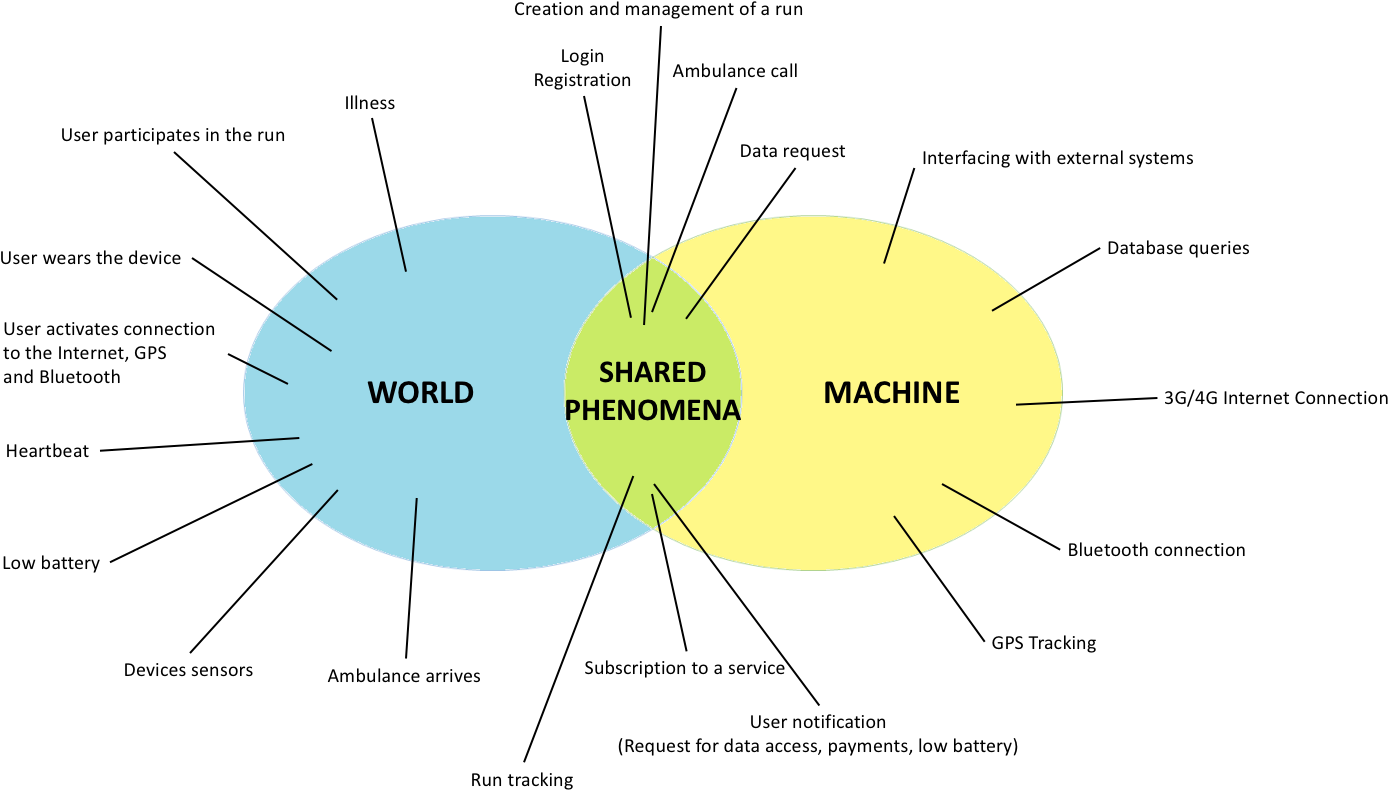
\includegraphics[width=\textwidth]{img/WorldMachine.png}
  \hspace{0.05\linewidth}
  \centering
  \caption{World and Machine model}
  \label{img:WandMmodel}
\end{center}
\end{figure}

\section{Definitions, Acronyms and Abbreviations}
\begin{itemize}
  \setlength{\itemindent}{-.4in}
  \item[] \textbf{API}: Application Programming Interface;
  \item[] \textbf{GPS}: Global Positioning System;
  \item[] \textbf{Organizer}: A registered user that organizes a run, defining date and path;
  \item[] \textbf{OS}: Operating System;
  \item[] \textbf{RASD}: Requirement Analysis and Specification Document;
  \item[] \textbf{Run}: An event that is organized by one organizer, at which one or more people can partecipate and that can be followed by one or more spectators;
  \item[] \textbf{Runner}: A registered user that enrols for a run;
  \item[] \textbf{Spectator}: Unregistered user that access to Track4Run to follow a run;
  \item[] \textbf{SSN}: Social Security Number;
  \item[] \textbf{System}: The software system-to-be, including all of its services;
  \item[] \textbf{Third party}: Any external organization that wants to access to data acquired by Data4Help;
  \item[] \textbf{UML}: Unified Modeling Language;
  \item[] \textbf{User}: Any person, registered or not, who accesses to one of the applications (for Data4Help there is a special user called \textit{Third party});
  \item[] \textbf{VAT}: Value Added Tax.
\end{itemize}

\section{Reference documents}
------------------ TODO ------------------

\section{Overview}
This document is structured as follows:
\begin{itemize}
  \setlength{\itemindent}{-.4in}
  \item[] \textbf{Section 1: Introduction}. A general introduction to the goals, the phenomena and the scope of the system-to-be. It aims giving general but exaustive information about what this document is going explain.
  \item[] \textbf{Section 2: Overall Description}.
  \item[] \textbf{Section 3: Specific Requirements}.
  \item[] \textbf{Section 4: Effort Spent}. A summary of the worked time by each member of the group.
\end{itemize}
At the end there is the bibliography.

\clearpage

%Overall Description
\chapter{Overall Description}
\section{Product Perspective}

\subsection{User Interfaces}\label{userInterfaces}

\subsubsection{Standard Users}
Standard users can use two different smartphone applications: \textit{AutomatedSOS} and \textit{Track4Run}.
Both of them should be very easy to use and should allow the user to connect the smartphone to the smartwatch or to the chosen device.
\textit{AutomatedSOS} is mainly used by elderly people so it should have large buttons and large writing and it shouldn't ask to the user to interact a lot with the device.
\textit{Track4Run} is mainly used by young people so it should be more interactive.
%% and allow the sharing of the track on social networks and other social options such as comparing race data with friends.
Standard users can also access services provided by TrackMe using a web application. Using it they can manage their accounts in a more comfortable way, verify requests for accessing their data, create new route and follow a race watching players position on the map (in \textit{Track4Run} service).

\subsubsection{Special Users}
Third parties who want to analyse data collected from \textit{Data4Help} can access the service using a web application.
The web application lets special users to insert a request for data.
If the request is accepted, it allows the download of the asked data.
The system should also offer an online support to help user in using the service.

\subsection{Hardware Interfaces}\label{hardwareInterfaces}
\begin{itemize}
\item Web applications (both the one for standard users and the one for special users) must be accessible using a computer with characteristic specified in Section \ref{hardwareLimitation}.
\item Smartphone on which the app will work must provide to the app an Internet connection used to send data to TrackMe servers and must have a GPS antenna built in.
The wearable device must also integrate a reasonably precise heartbeat sensor and a pressure sensor.
\end{itemize}

\subsection{Software interfaces}\label{softwareInterfaces}
\begin{itemize}
\item Web applications (both the one for standard users and the one for special users) must be compatible with the most popular browsers such as Google Chrome, Mozilla Firefox, Microsoft Edge, Apple Safari;
\item	Mobile apps for standard users must be available for both iOS and Android devices and must be compatible with most of the smartwatch and other health devices available on the market regardless of the operating system used by the device (using the API made available to programmers by producers);
\item	Application backend stores collected data in a relational DBMS;
\item	 Web applications show data by accessing the relational DBMS;
\item	 Web applications for third parties has to interface also with a payments broker in order to receive money from companies who want to get data from the system;
\item Web application and Track4Run have to interface also with Maps in order to generate the path for the run and to virtually follow a run;
\item \textit{AutomatedSOS} has to interface with ambulance call external service.
\end{itemize}
\clearpage

\section{Product Functions}
The system is composed by several applications.
\subsubsection{AutomatedSOS}
\textit{AutomatedSOS} is designed for elderly people and offers a feature that makes an automatic call for help if it detects a dangerous state of health.
To use this app, few user interactions are required.
In particular the user can:
\begin{itemize}
\item Register to the service;
\item Log-in to the service;
\item Respond to requests to access to his/her personal data by a third party;
%%\item Report a false alarm following an emergency call with an alert to the nearest ambulance;
\item Manage personal account and send a request to delete all the acquired data;
\item Connect an health device such as smartwatch, smart band, heart rate sensors with Bluetooth;
\item Pause data monitoring.
\end{itemize}
The app will autonomously monitor the health status of the user and make an emergency call to the nearest ambulance in case of emergency.

\subsubsection{Track4Run}
\textit{Track4Run} is designed to track athletes participating in a run.
Using it the user can:
\begin{itemize}
\item Register to the service;
\item Log-in to the service;
\item Respond to requests to access to his/her personal data by a third party;
\item Manage his/her personal account;
\item Connect an health device such as smartwatch, smart band, heart rate sensors with Bluetooth;
\item Pause data monitoring.
%%\item Share performance data via popular social networks such as Facebook, Instagram, Twitter, etc.
\end{itemize}
The app will autonomously track the health status and the position of the athlete.

\subsubsection{Web application for standard users}
Using it they can:
\begin{itemize}
\item Register to the service;
\item Log-in to the service;
\item Respond to requests to access to their personal data by a third party;
\item Manage personal account;
\item Crate a path to be used in \textit{Track4Run};
%%\item Send an invitation to join in a run;
\item Follow a competition watching the position of the athletes on the map.
\end{itemize}

\subsubsection{Web application for special users}
Using it they can:
\begin{itemize}
\item Register to the service;
\item Log-in to the service;
\item Send a request to access to the data of a standard user;
\item Send a request to access to the data of a group of people;
\item Manage past requests;
\item Download data obtained after a request has been accepted and paid.
\end{itemize}


\begin{figure}[H]
\begin{center}
  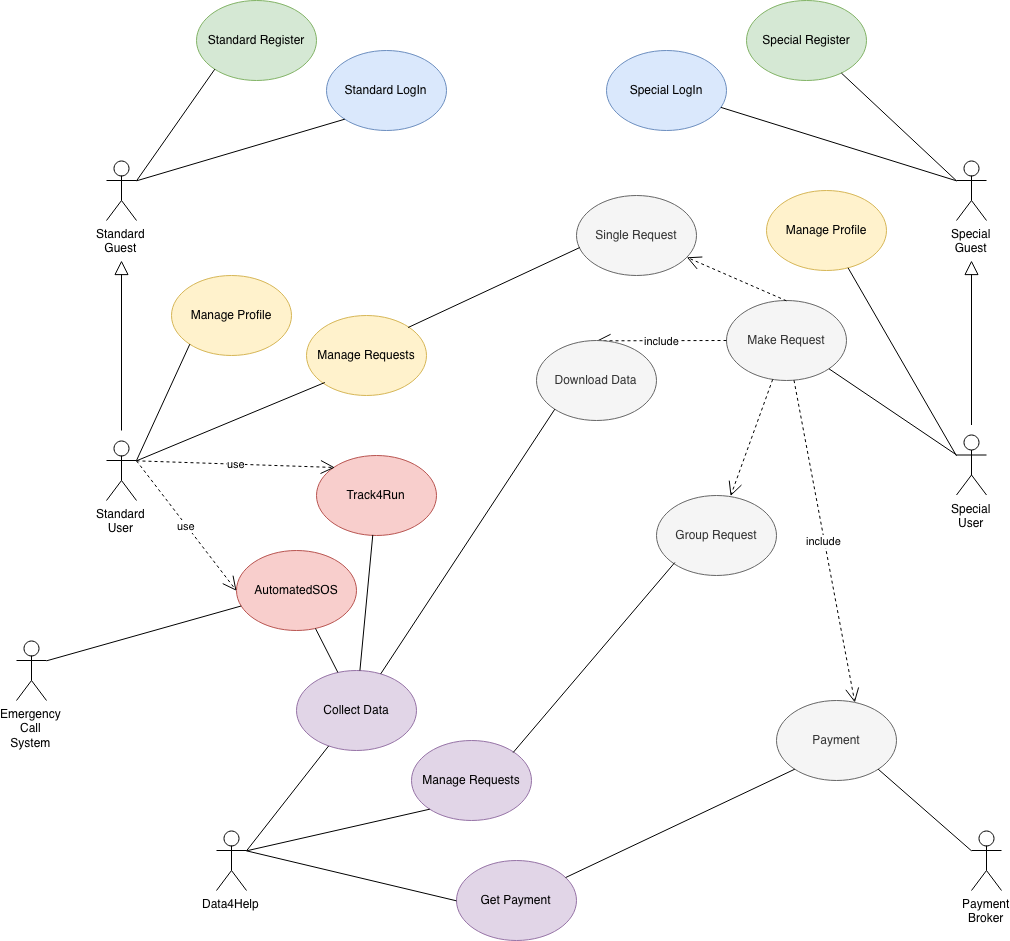
\includegraphics[width=\textwidth]{img/UseCase_Diagram.png}
  \hspace{0.05\linewidth}
  \centering
  \caption{Use Case Diagram}
  \label{img:UseCase_Diagram}
\end{center}
\end{figure}

\section{User Characteristics}
Those applications have different targets.

\subsubsection{AutomatedSOS}
This mobile app is thought for elderly people. It is not necessary that the user is a “tech addicted” because a familiar can setup the system for him/her and than it will work autonomously.

\subsubsection{Track4Run}
This mobile app is thought for athletes. It is most dedicated to young people who use frequently tech products.

\subsubsection{Third party WebApp}
This application is thought for companies who want to analyse data collected by the app. They could be statistics or pharmaceutical companies, hospitals, etc.

\section{Constraints}

\subsection{Anonymous data collection}
Companies who want to analyse data from a group of people without asking the permission to every single person must make a request for anonymized data of a group of at least 1000 people.

\subsection{Privacy}
Before allowing a company to access to user’s data, it is necessary to get a formal permission by the user.

\subsection{Regulatory Policies}
When a new user registers to the service he must accept the privacy policy in order to use the application.
He must be informed about personal and sensible data collection that is carried out by the applications (his/her position and his/her health parameters).
%%In every moment the user can ask TrackMe to delete all the collected data about him.
All the collected data must be kept safe and must not be accessible by unauthorized person.
Also, third parties who access the service must guarantee the security of the data.
The whole process must comply with the GDPR regulations for the protection of users' personal data.
\clearpage

\subsection{Hardware limitations}\label{hardwareLimitation}
In order to use the service, user’s hardware should comply to these minimum requirements:
\subsubsection{Mobile application}
\begin{itemize}
  \item Smartphone:
  \begin{itemize}
    \item iOS or Android operative system;
    \item UMTS/4G Internet connection with a minimum speed of 1Mb/s;
    \item Bluetooth antenna;
    \item GPS antenna;
    \item 300 Mb available memory;
    \item Dual-core processor;
    \item 1 Gb RAM.
  \end{itemize}
  \item Smartwatch / other health device:
  \begin{itemize}
    \item Bluetooth antenna;
    \item Heartbeat sensor;
    \item Pressure sensor.
  \end{itemize}
\end{itemize}

\subsubsection{Web application}
\begin{itemize}
  \item Computer:
  \begin{itemize}
    \item Internet connection with a minimum speed of 1Mb/s;
    \item Browser application;
    \item 720p monitor resolution.
  \end{itemize}
\end{itemize}

\subsection{Parallel operation}
The system must guarantee the operation of the system in case of simultaneous use of the mobile app by at least 100,000 users and simultaneous use of the web app by at least 10,000 users.
Consequently, the DBMS must be able to process a large number of simultaneous transactions.

\subsection{Reliability requirement}
The system reliability, seen as the probability that components and performances will meet the requirement during a specified period of time, must be at least 95\%, considering a period of one month.

\subsection{Availability requirement}
The system should be available 24/7 in order to guarantee the services and manage emergency situations.

\subsection{Criticality of the system}
\subsubsection{AutomatedSOS}
An error in the system could result in an unnecessary call for an ambulance or in a failure to call an ambulance.
\subsubsection{Track4Run}
An error in the system could cause a non-optimal use of the service.

\section{Assumptions and Dependencies}
From now on the following assumptions are given for guaranteed:
\begin{enumerate}
  \item Users of the app have a phone with an iOS or Android operating system;
  \item Users of the app have a phone with working GPS module with an uncertain of \begin{math} \pm1 \end{math} meter;
  \item All users enjoy a stable Internet connection;
  \item Users accept or refuse a request for access to their data within 24 hours from when it has been recievd. After this period the request is considered rejected;
  \item Each user is identified with his/her/its e-mail;
  \item Once a request is accepted by a user, the system provides the applicant with the required data within 24 hours;
  %%\item Users enter the correct data during registration.
  \item The user autonomously recharges the smartphone and the smartwatch when its battery is low;
  \item A user cannot participate in two races at the same time;
  \item Every request for access to user's personal data from a third parties must be explicitly accepted by the user;
  \item When a third party accesses to the personal data of a user it is responsible for any unauthorized disclosure of data.
\end{enumerate}

\vspace{1cm}

Behavioural during devices recharge time:
\begin{enumerate}
  \item If the smartphone is charging in a fixed position near the user, the wearable device remains connected via Bluetooth to the smartphone and the \textit{AutomatedSOS} service is not interrupted;
  \item If the smartphone is charging in a fixed position, the \textit{Track4Run} service is interrupted;
  \item If the smartphone is charging using a transportable battery, all the services keep working;
  \item If the wearable device is charging, the service \textit{AutomatedSOS} is interrupted;
  \item If the wearable device is charging, the service \textit{Track4Run} keep working (available only data about position);
\end{enumerate}

\section{Future Extensions}
The addition of new features will be evaluated in the future. The possible proposals are:
\begin{enumerate}
  \item The creation of a new application with the purpose of collecting user data, without offering services such as \textit{AutomatedSOS} and \textit{Track4Run}. Users will be paid to use the application consistently. This operation considerably increases the number of users and also collects data from those subjects that are currently excluded (people who are not elderly and do not practice sports);
  \item The possibility for the user to share their sanitary facilities for free with their doctor.
\end{enumerate}

\clearpage

%Specific Requirements
\chapter{Specific Requirements}\label{ch:section3}
\section{External Interface Requirements}

\subsection{User Interfaces}
The user interfaces of \textit{AutomatedSOS} and \textit{Track4Run} must be intuitive and user-friendly in order to permit an easy interaction with all the services offered by the systems.\\
Moreover both the application and the web site must support multiple languages.

\subsection{Hardware Interfaces}

\subsection{Software Interfaces}

\subsection{Communication Interfaces}

\clearpage
\section{Functional Requirements}

\subsection{Individual Sign In}
\myparagraph{Purpose}
Anyone who wants to subscribe to one or both services offered by \textit{Data4Help} must go through the registration process, which can be carried out either through \textit{AutomatedSos} and \textit{Track4Run} apps or through the web site.
The process requires exactly the same steps regardless the platform through which it is carried out:
\begin{enumerate}
  \item The new user is required to fill in all the fields in which she/he is asked for his name, his surname, his date of birth, his city of birth, his city of residence and a valid e-mail address;
  \item The user must accept the conditions regarding his privacy, in particular the collection of his data by \textit{Data4Help} and the sharing of them in anonymous way with third parties.
\end{enumerate}
After that the system will check the correctness of the inserted data, in particular it will check that the user isn't already registerd and that the inserted e-mail isn't already used by someone else. If the result of this control is positive the registration is authorized and the user will recive a confermation e-mail to the specified e-mail address with the password she/he has to use to access to all \textit{Data4Help} services.

\myparagraph{Scenario 1}
Sara would like to register her grandmother to \textit{AutomatedSos} to not worry about her helth status when they are not together. She opens the browser on his personal computer and search for \textit{Data4Help} web site, then she clicks on the "\textit{Sign In}" button, which is located in the main page. She passes through the steps of the registration process, inserting his grandmother data and accepting the required conditions. Finally, if the inserted data are accepted by the system, she recives the confirmation e-mail.

\myparagraph{Scenario 2}
Marco wuold like to organize an amateur run with his friends and remembers that someone told him something about a new application called \textit{Track4Run} so he decides to try it. He downloads the app on his smartphone and turn it on. The first page that is shown to him contains the "\textit{Sign In}" button and the "\textit{Log In}" one, he presses on the first one and starts his registration process. He doesn't use his personal e-mail address, but an e-mail address he has in common with his brother that they usually use to make purchase online. Unexpectedly he is informed by the system that the insert e-mail is already registered in the database and so he has to change it and this time he inserts his personal e-mail address. This time the registration is succesfull and he recives the confermation e-mail.

\myparagraph{Use Case}
The Individual Sign In is analyzed in Table \ref{table:individualSignInTable}.

\myparagraph{Functional requirements}
\begin{enumerate}
  \item The system must not accept an e-mail address that is already used by an already registered user;
  \item The system must not authorize the registration untill all the fields are filled up;
  \item The system must not authorize the registration untill the required conditions aren't accepted;
  \item The system must send the confirmation e-mail to the inserted e-mail address with the password when "\textit{Submit}" button is clicked only if all the inserted data are acceptable and the required conditions has been accepted;
  \item The system must let the \textbf{Individual user to be} leave the registration process at anytime.
\end{enumerate}

\begin{center}
\begin{table}
\begin{tabular}{ | l | p{0.75\linewidth} | }
  \hline
    Actor & \textbf{Individual user to be} \\ \hline
    Goal & \textbf{[G.1]} \\ \hline
    Input Condition & A person wants to subscribe to one of \textit{Data4Help} services \\ \hline
    Event Flow & \begin{minipage}[t]{0.7\textwidth}
      \begin{enumerate}
        \item The \textbf{Individual user to be} opens the main page of \textit{Data4Help} web site from his personal computer or of \textit{AutomatedSos} or \textit{Track4Run} apps from his smartphone;
        \item The \textbf{Individual user to be} clicks on "\textit{Sign in}" button;
        \item The system shows the form the \textbf{Individual user to be} has to fill up;
        \item The \textbf{Individual user to be} fills up the form with his name, his surname, his date of birth, his city of birth, his city of residence and an e-mail address;
        \item The \textbf{Individual user to be} accepts the required conditions;
        \item The \textbf{Individual user to be} clicks on "\textit{Submit}" button;
        \item The system checks wheter the inserted information are acceptable or not;
        \item The \textbf{Individual user to be} recives a confirmation e-mail containing the password he has to use to access to all \textit{Data4Help} services.
      \end{enumerate}
    \smallskip
  \end{minipage} \\ \hline
  Output Condition & The system tells the \textbf{Individual user to be} that his registration is completed \\ \hline
  Exceptions & \begin{minipage}[t]{0.7\textwidth}
    \begin{itemize}
      \smallskip
      \item If functional requirements 1 or 2 are not satisfied the process goes back to step 4;
      \item If functional requirement 3 is not satisfied the process goes back to step 5;
      \item If the \textbf{Individual user to be} decides to leave the registration process this one is aborted.
    \end{itemize}
    \smallskip
  \end{minipage}  \\ \hline
\end{tabular}
\caption{Individual Sign In use case}
\label{table:individualSignInTable}
\end{table}
\end{center}


\clearpage

%Specific Requirements
\chapter{Alloy}
\begin{figure}[H]
  \begin{center}
  	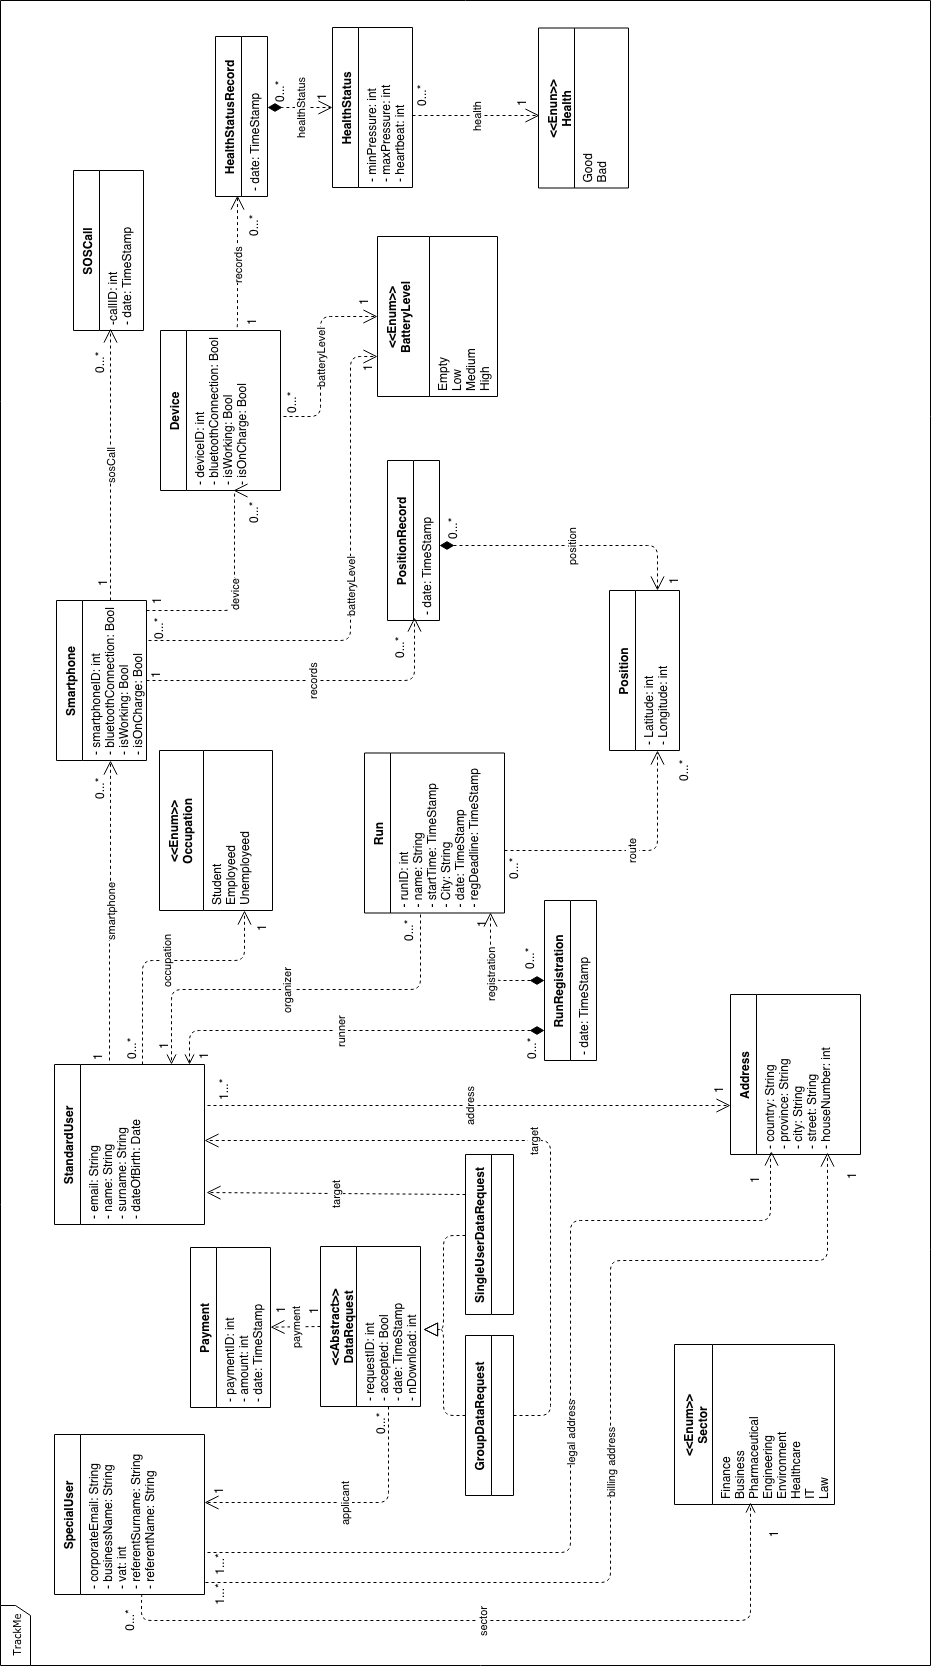
\includegraphics[height=0.45\paperheight]{./img/Class_Diagram.png}
		\caption{\textit{Class diagram} of the structure of the system-to-be.}
    \hspace{0.05\linewidth}
    \centering
		\label{classDiagram}
    \end{center}
\end{figure}

\newpage

% Settings for Alloy code listing.
\lstset{
    language=alloy,
    numbers=left,
    numberstyle=\tiny,
    stepnumber=2,
    tabsize=4,
    keywordstyle=\color{alloy-keyword}\bfseries,
    commentstyle=\color{alloy-comment},
    stringstyle=\color{alloy-string},
    basicstyle=\small\fontfamily{pcr}\selectfont, % Courier font family
}

% Includes the Alloy model file.
\lstinputlisting{./files/Alloy.als}
%\vfill

\clearpage

%Specific Requirements
\chapter{Effort Spent}
\section{Michele Gatti}

%Space
\smallskip
\begin{center}
\begin{tabular}{ | p{0.75\linewidth} | l | }
  \hline
    \textbf{Task} & \textbf{Hours }\\ \hline
    Purpose and Goals & 1 \\ \hline
    Product Perspective and Product Functions & 6 \\ \hline
    User Characteristics and Constraints & 2 \\ \hline
    Assumptions and Dependencies & 3 \\ \hline
    The World and the Machine & 3 \\ \hline
    Team revision & 1 \\ \hline
    Class Diagram & 6 \\ \hline
    Alloy & 14 \\ \hline
    Team work & 2 \\ \hline
    \textbf{Total} & \textbf{38} \\ \hline
\end{tabular}
\end{center}
%Space
\smallskip


\section{Federica Gianotti}

%Space
\smallskip
\begin{center}
\begin{tabular}{ | p{0.75\linewidth} | l | }
  \hline
    \textbf{Task} & \textbf{Hours }\\ \hline
    Purpose and Goals & 4 \\ \hline
    Scope, Definitions, Acronyms and Abbreviations & 2 \\ \hline
    Team revision & 1 \\ \hline
    Functional Requirements & 14 \\ \hline
    Functional Requirements and Mockup revision & 4 \\ \hline
    Activity Diagrams & 4 \\ \hline
    Class Diagram & 2 \\ \hline
    Alloy & 2 \\ \hline
    Team work & 2 \\ \hline
    Final revision & 3 \\ \hline
    \textbf{Total} & \textbf{38} \\ \hline
\end{tabular}
\end{center}
%Space
\smallskip

\section{Mathyas Giudici}

%Space
\smallskip
\begin{center}
\begin{tabular}{ | p{0.75\linewidth} | l | }
  \hline
    \textbf{Task} & \textbf{Hours }\\ \hline
    \textit{GitHub and LaTeX setup} & \textit{2} \textsuperscript{*} \\ \hline
    Purpose and Goals & 2 \\ \hline
    Scope, Definitions, Acronyms and Abbreviations & 2 \\ \hline
    Team revision & 1 \\ \hline
    Functional Requirements & 14 \\ \hline
    User Interface Mockup & 4 \\ \hline
    Functional Requirements and Mockup revision & 4 \\ \hline
    Activity Diagrams & 3 \\ \hline
    Class Diagram & 2 \\ \hline
    Alloy & 2 \\ \hline
    Team work & 2 \\ \hline
    Final revision & 2 \\ \hline
    \textbf{Total} & \textbf{38} \\ \hline
\end{tabular}
\end{center}

\textsuperscript{*} : GitHub and LaTeX setup hours are not counted in the total of the hours

\clearpage

\clearpage


\begin{thebibliography}{9}

  \bibitem{ieee-29148}
	ISO/IEC/IEEE 29148:2011 \emph{Systems and software engineering - Life cycle processes - Requirements engineering}

  \bibitem{ieee-830}
	IEEE 830:1998 \emph{Recommended Practice for Software Requirements Specifications}

  \bibitem{world-machine}
  M.Jackson \& P. Zave, \emph{The World and The Machine}, 1995

  \bibitem{se-assignments}
  Elisabetta Di Nitto - Software Engineering 2 Slides (AY 2018/2019) \emph{Project goal, schedule and rules}

\end{thebibliography}


\end{document}
